\section{Zusammenfassung und Diskussion}

In Versuch 255 untersuchten wir unter Einsatz der Drehkristallmethode mit einem LiF- und einem NaCl-Kristall das Spektrum der Röntgenstrahlung einer Röntgenröhre mit Molybdänanode. Das Röntgenspektrum zeichnet sich durch ein kontinuierliches Spektrum aus, welches durch Bremsstrahlung erzeugt wird, dem ein diskretes Spektrum, erzeugt durch Ionisation im Anodenmaterial der Röntgenröhre, überlagert ist.

Wir untersuchten zunächst das Röntgengenspektrum, aufgezeichnet in der Drehkristallmethode mit einem LiF-Kristall. Dieses ist noch einmal in \abbref{fig:spektrum_lif_komplett_zsmf} abgebildet.

\begin{figure}[H]
  \centering
  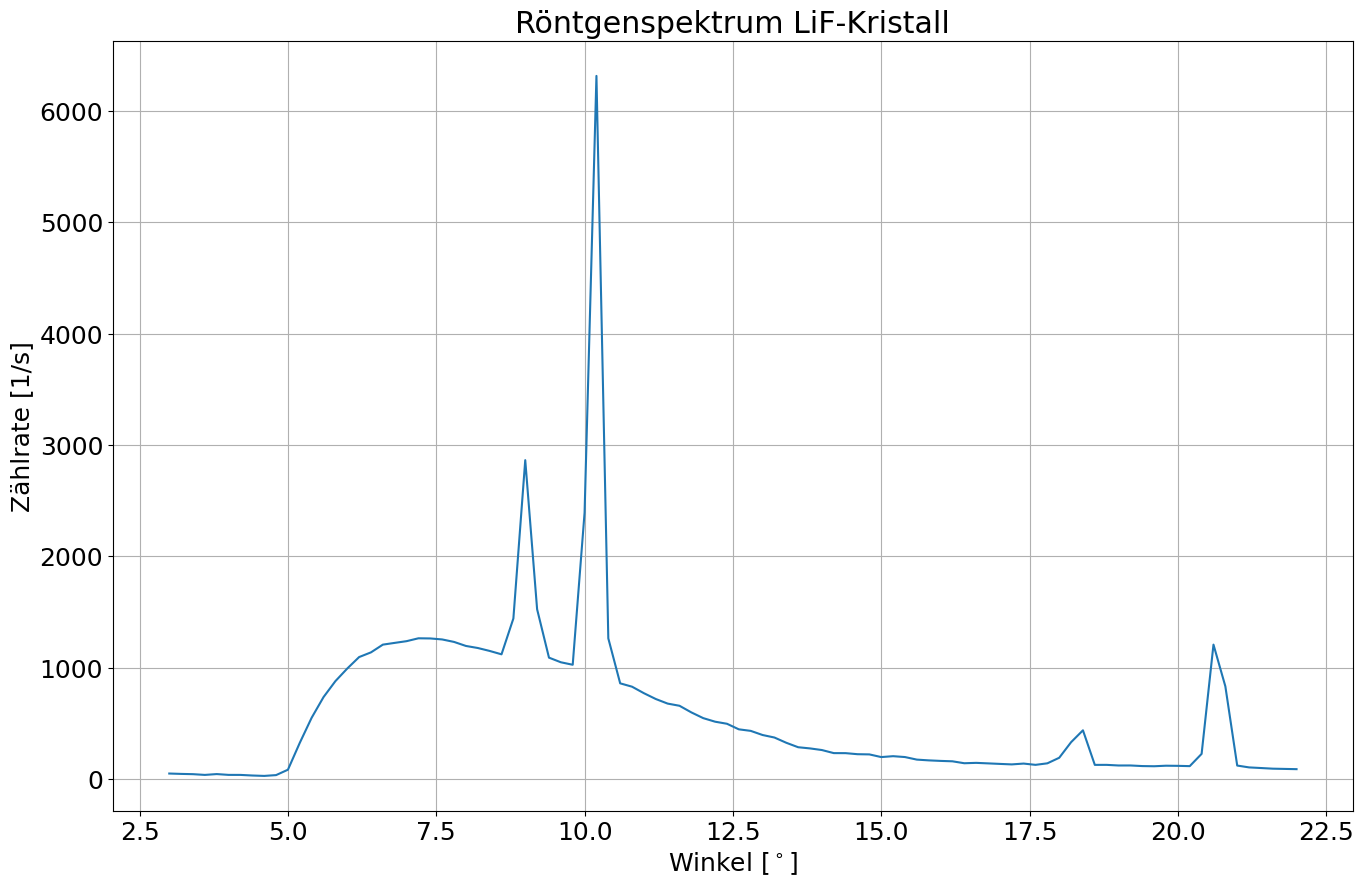
\includegraphics[width=.9\textwidth]{files/plots/spektrum_lif_komplett.png}
  \caption{Röntgenspektrum mit LiF-Kristall}
  \label{fig:spektrum_lif_komplett_zsmf}
\end{figure}

Im ersten Teil bestimmten wir die Grenzwellenlänge des Spektrums, also den Punkt am kurzwelligen Ende, an dem das Spektrum erster Ordnung einsetz. Hierzu ermittelten wir einen Wert von
\begin{align}
  \lambda_{Grenz} = (34.33 \pm 3.08) \si{\pico\meter}.
\end{align}

Aus der Grenzwellenlänge berechneten wir für das Planck'sche Wirkungsquantum einen Wert von
\begin{align}
  h = (6.4 \pm 0.6) \cdot 10^{-34} \si{\joule\second}.
\end{align}

Dieser Wert weicht von dem in der Praktikumsanleitung gegebenen Wert von $h_{lit} = 6.6261 \cdot 10^{-34} \si{\joule\second}$ um $0.36\sigma$ ab. Diese Abweichung ist sehr gering und kann als nicht signifikant angesehen werden.

Am Ende dieses Aufgabenteils bestimmten wir noch den Winkel des Drehkristalls, ab dem das Spektrum zweiter Ordnung einsetzt. Hierfür kamen wir auf einen Wert von
\begin{align}
  \vartheta_{0,2. Ord} = (9.813 \pm 0.016)\si{\degree}.
\end{align}

Im zweiten Versuchsteil betrachteten wir die Lagen der $K_{\alpha}$- und $K_{\beta}$-Linien erster und zweiter Ordnung, welch durch Ionisation in der Molybdänanode erzeugt werden, genauer. Für alle vier Linien bestimmten wir mittels eines Fits einer Gaußkurve an die Daten die Winkelposition des Drehkristalls, an welcher diese auftreten, die zugehörige Standardabweichung, sowie deren Halbwertsbreite. Mithilfe des Bragg'schen Gesetztes berechneten wir aus den Winkeln wieder die zugehörigen Wellenlängen und bildeten einen Mittelwert über die Linien erster und zweiter Ordnung. Die Ergebnisse sind noch einmal in \tabref{tab:k_linien_zsmf} zusammengefasst. Die Literaturwerte für die Positionen der Linien stammen ebenfalls aus der Praktikumsanleitung.

\begin{table}[H]
  \centering
  \begin{tabular}{c|c|c|c|c|c}
    Linie & Ordnung & $\lambda$ $[\si{\pico\meter}]$ & $\overline{\lambda}$ $[\si{\pico\meter}]$ & $\lambda_{Lit}$ $[\si{\pico\meter}]$ & Abweichung\\\hline
    %
    \multirow{2}{*}{$K_\alpha$} & 1 & $71.27 \pm 0.19$ & \multirow{2}{*}{$71.17 \pm 0.12$} & \multirow{2}{*}{$71.1$} & \multirow{2}{*}{$0.65\sigma$}\\
     & 2 & $71.07 \pm 0.12$ & & & \\\hline
    %
    %
    \multirow{2}{*}{$K_\beta$} & 1 & $63.27 \pm 0.05$ & \multirow{2}{*}{$63.27 \pm 0.14$} & \multirow{2}{*}{$63.1$} & \multirow{2}{*}{$1.29\sigma$}\\
     & 2 & $63.27 \pm 0.10$ & & & 
  \end{tabular}
  \label{tab:k_linien_zsmf}
\end{table}

Wir können sehen, dass auch hier wieder die Abweichung sehr gering ausfällt.

Im darauf folgenden Versuchsteil betrachteten wir die Auswirkungen der an der Röntgen-röhre anliegenden Beschleunigungsspannung genauer. Dazu stellten wir den Drehkristall auf einen festen Winkel von $7.5\si{\degree}$ und nahmen die Zählraten für Beschleunigungsspannungen im Bereich von $20$ bis $35 \si{\kilo\volt}$ auf. Die Zählraten zeigten ab einem bestimmten Punkt einen mit der Spannung linearen Anstieg auf. Mittels einer Extrapolation ermittelten wir die Spannung, ab welcher die ersten Ereignisse gezählt wurde auf
\begin{align}
  U_{0} = 22.872 \pm 1.025 \si{\kilo\volt}.
\end{align}

Nach dem Bragg'schen Gesetz entsprach der eingestellte Winkel von $7.5\si{\degree}$ einer Wellenlänge von $(52.6 \pm 0.4)\si{\pico\meter}$. Mit diesen Werten konnten wir erneut einen Wert von
\begin{align}
  h = (6.43 \pm 0.30) \cdot 10^{-34} \si{\joule\second}
\end{align}
ermitteln. Dieser Wert weicht um $0.69\sigma$ vom Literaturwert aus der Praktikumsanleitung ab. Der berechnete Wert liegt zwar etwas näher am Literaturwert, allerdings haben wir nun einen kleineren Fehler, wodurch die größere $\sigma$-Abweichung zustande kommt.

Für den letzten Versuchsteil führten wir die Aufzeichnung des Röntgengenspektrums noch einmal mit einem NaCl-Kristall in einem Winkelbereich von $3\si{\degree}$ bis $18\si{\degree}$ durch. Dieser Bereich des Spektrums ist noch einmal in \abbref{fig:spektrum_nacl_komplett_zsmf} zu sehen. Aus den Daten ermittelten wir erneut die Winkelpositionen der $K_{\alpha}$- und $K_{\beta}$-Linien erster Ordnung. Diese identifizierten wir mit den Wellenlängen der $K_{\alpha}$- und $K_{\beta}$-Linien aus Versuchsteil 2. Damit konnten wir, erneut durch eine umgestellte Form des Bragg'schen Gesetzes, den Netzebenenabstand $d$ berechnen.

\begin{figure}[H]
  \centering
  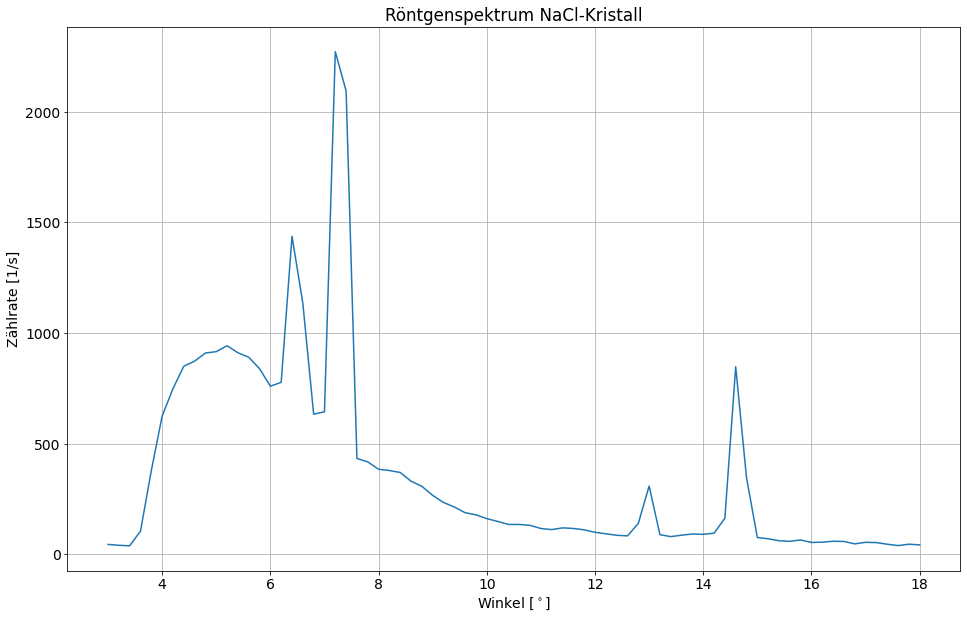
\includegraphics[width=.9\textwidth]{files/plots/spektrum_nacl_komplett.png}
  \caption{spektrumnaclkomplett}
  \label{fig:spektrum_nacl_komplett_zsmf}
\end{figure}

Die Ergebnisse sind noch einmal in der folgenden \tabref{tab:d_calc_zsmf} zusammengefasst.

\begin{table}[H]
  \centering
  \begin{tabular}{c|c|c|c|c}
    Linie & Winkel $\si{\degree}$ & $\lambda$ $[\si{\pico\meter}]$ (Aufg. 2) & $d$ $[\si{\pico\meter}]$ & $\overline{d}$ $[\si{\pico\meter}]$\\\hline
    $K_{\alpha}$ & $7.29 \pm 0.05$ & $71.17 \pm 0.12$ & $280.4 \pm 1.8$ & \multirow{2}{*}{$280.8 \pm 1.5$}\\
    $K_{\beta}$ & $6.46 \pm 0.05$ & $63.27 \pm 0.14$ & $281.2 \pm 2.3$ &
  \end{tabular}
  \label{tab:d_calc_zsmf}
\end{table}

Der Netzebenenabstand $d$ entspricht bei NaCl gerade der halben Gitterkonstante, somit konnten wir diese durch einfaches Verdoppeln des Wertes zu
\begin{align}
  a = (561.6 \pm 2.9) \si{\pico\meter}
\end{align}
berechnen. In der Literatur ist die Gitterkonstante von NaCl mit $a_{Lit} = 564\si{\pico\meter}$\footnote{https://de.wikipedia.org/wiki/Natriumchlorid-Struktur.} angegeben. Der von uns berechnete Wert weicht von diesem um etwa $0.84\sigma$ ab.

Zu guter Letzt verwendeten wir den soeben berechneten Netzebenenabstand zur Berechnung der Avogadrokonstante. Hierbei kamen wir auf einen Wert von
\begin{align}
  N_A = (6.10 \pm 0.10) \cdot 10^{23} \si{\per\mol}.
\end{align}

In der Praktikumsanleitung ist die Avogadrokonstante mit einem Wert von $N_{A,Lit} = 6.0221 \cdot 10^{23}\si{\per\mol}$ angegeben. Unser Wert weicht von diesem um $0.82\sigma$ ab.

Allgemein können wir sehen, dass die Abweichungen der von uns berechneten Werte von den Literaturwerten in einem Bereich um $1\sigma$ bewegen, also sehr gering sind. Ein Grund für die dennoch auftretenden Abweichungen könnte zum einen dadurch zustande kommen, dass wir die Winkelbereiche immer noch in vergleichsweise großen Schritten aufgenommen haben. Somit fällt es schwer, die genaue Position der diskreten $K$-Linien zu ermitteln und auch die Fehlerabschätzung ist nur sehr grob möglich. Weiter ist zu bemerken, dass sich die $K$-Linien eigentlich, wie in der Einleitung erwähnt, noch durch eine Feinstrukturaufspaltung auszeichnen, welche eine Entartung der Drehimpuls- und Spinquantenzahl miteinbezieht. Diese haben wir in unseren Berechnungen nicht beachtet und auch einige der verglichenen Literaturwerte sind lediglich Mittelwerte über die Aufspaltung.